\chapter{Аналитическая часть}
\section{Компоненты компилятора}
Компилятор является сложной программной системой, состоящей из нескольких взаимосвязанных компонентов. Типичная архитектура компилятора включает в себя следующие основные составляющие:

\begin{enumerate}
    \item Frontend (передняя часть) - этот компонент отвечает за преобразование исходного кода программы на высокоуровневом языке в промежуточное представление. Он включает в себя следующие этапы:
    \begin{itemize}[label = ---]
        \item Препроцессор - выполняет предварительную обработку исходного текста, такую как раскрытие макросов, обработка директив препроцессора и т.д.
        \item Лексический анализатор - выполняет разбиение входного текста на лексемы (токены) в соответствии с правилами грамматики.
        \item Синтаксический анализатор - строит синтаксическое дерево, основываясь на потоке лексем, полученных на предыдущем этапе.
        \item Семантический анализатор - проверяет семантическую корректность программы, определяет типы, области видимости, связывает объявления и использования идентификаторов.
        \item Генератор промежуточного представления - на основе синтаксического дерева и результатов семантического анализа генерирует промежуточное представление программы, которое будет использоваться на следующих этапах компиляции.
    \end{itemize}
    \item Middle-end (средняя часть) - этот компонент отвечает за оптимизацию промежуточного представления программы. Он выполняет различные анализы и преобразования, направленные на улучшение характеристик генерируемого кода, таких как время выполнения, размер, энергопотребление и т.д.
    \item Backend (задняя часть) - этот компонент отвечает за генерацию машинного кода (или ассемблерного) для целевой аппаратной платформы. Он использует оптимизированное промежуточное представление и выполняет следующие основные этапы:
    \begin{itemize}[label = ---]
        \item Регистровый распределитель - распределяет переменные программы по доступным регистрам процессора.
        \item Генератор кода - генерирует машинные инструкции, соответствующие промежуточному представлению.
        \item Оптимизатор кода - выполняет дополнительные оптимизации на уровне машинных инструкций.
    \end{itemize}
\end{enumerate}

Рисунок \ref{img:1.1} иллюстрирует основные фазы работы компилятора, описанные выше.

\captionsetup{justification=centering,singlelinecheck=off}
\begin{figure}[h!]
	\centering
		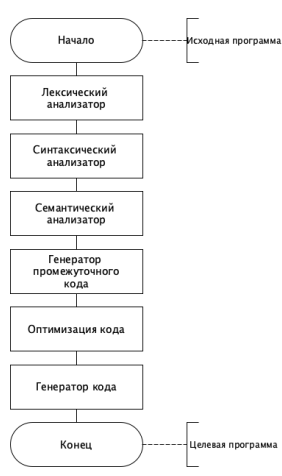
\includegraphics[,scale=1.2]{./img/1.1.png}
		\caption{Фазы компилятора.}  
		\label{img:1.1}
\end{figure}

Взаимодействие этих компонентов обеспечивает эффективную трансляцию исходного кода программы в машинно -зависимый двоичный код, готовый к выполнению на целевой аппаратной платформе
\subsection{Препроцессор}
Препроцессор является первым звеном в цепочке компиляции, выполняя ряд важных функций по подготовке входных данных для последующих этапов:
\begin{enumerate}
    \item Обработка директив препроцессора:
    \begin{itemize}[label = ---]
        \item Раскрытие макросов с параметрами и без.
        \item Включение внешних файлов.
        \item Реализация условной компиляции.
        \item Управление символами препроцессора.
    \end{itemize}
    \item Преобразование исходного текста:
    \begin{itemize}[label =---]
        \item Удаление комментариев.
        \item Нормализация белых пробелов.
        \item Обработка директив языковых расширений.
    \end{itemize}
    \item Формирование потока лексем для последующего лексического анализа.
\end{enumerate}

\begin{lstlisting}[label=1,caption=До препроцессинга]
#include <stdio.h>

#define MAX_SIZE 100

int main() {
#ifdef DEBUG
    printf("Debugging mode enabled.\n");
#endif
    int arr[MAX_SIZE];
    // Заполнение массива
    for (int i = 0; i < MAX_SIZE; i++) {
        arr[i] = i;
    }
    return 0;
}
\end{lstlisting}

Рассмотрим пример работы препроцессора (см. Листинг 1) на программе на языке C, которая делает следующее:
\begin{itemize}[label = ---]
    \item Создает массив arr размером 100 элементов.
    \item Заполняет этот массив числами от 0 до 99.
    \item Если определен макрос DEBUG, выводит сообщение "Debugging mode enabled".
\end{itemize}

\begin{lstlisting}[label = 2, caption=После препроцессинга]
    int main() {
    printf("Debugging mode enabled.\n");
    int arr[100];
    // Заполнение массива
    for (int i = 0; i < 100; i++) {
        arr[i] = i;
    }
    return 0;
}
\end{lstlisting}

В результате работы препроцессора (см. Листинг \ref{2}):
\begin{enumerate}
    \item Директива \#include <stdio.h> была заменена на подключение соответствующей библиотеки.
    \item Макрос \#define MAX\_SIZE 100 был раскрыт, заменив все вхождения MAX\_SIZE на значение 100.
    \item Директива \#ifdef DEBUG и соответствующий блок вывода были сохранены, так как условие DEBUG было определено.
    \item Комментарии остались без изменений.
\end{enumerate}
Таким образом, препроцессор выполнил обработку директив, раскрытие макросов и подготовил финальный исходный код для последующих этапов компиляции.

Следовательно, препроцессор играет ключевую роль в подготовке и трансформации исходного кода программы, обеспечивая необходимую входную информацию для следующих этапов компиляции.

\subsection{Лексический анализатор}
Лексический анализ – это критическая процедура в разработке компилятора, отвечающая за преобразование входного потока символов в последовательность токенов. Этот процесс, также известный как ”токенизация группирует определенные терминальные символы в лексемы в соответствии с заданными правилами, обычно выраженными через регулярные выражения или конечные автоматы.

Основные функции лексического анализатора включают:
\begin{itemize}
    \item Удаление пробелов и комментариев из входного потока. Например, строка x = 10. 10 будет преобразована в последовательность токенов без комментария.
    \item Идентификация и формирование числовых констант из последовательностей цифр. Например, 42 или 3.14 будут распознаны как числовые литералы.
    \item Распознавание идентификаторов и ключевых слов языка. Например, var, if, return будут определены как ключевые слова языка, а myVariable как идентификатор.
\end{itemize}

\captionsetup{justification=centering,singlelinecheck=off}
\begin{figure}[h!]
	\centering
		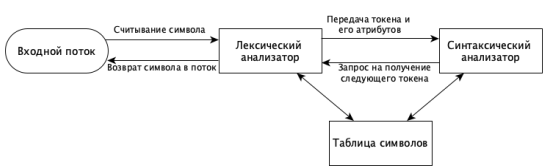
\includegraphics[,scale=1]{./img/1.2.png}
		\caption{Лексический анализатор.}  
		\label{img:1.2}
\end{figure}

Лексический анализатор находится между входным потоком и синтаксическим анализатором, как показано на рисунке \ref{img:1.2}. Он считывает символы из входного потока, группирует их в лексемы и передает последующим стадиям
9компиляции токены, образованные из этих лексем.

Например, последовательность символов var x = 42; будет разбита лексическим анализатором на следующие токены:
\begin{itemize}[label = ---]
    \item var (ключевое слово)
    \item x (идентификатор)
    \item = (оператор присваивания)
    \item 42 (числовая константа)
    \item ; (разделитель)
\end{itemize}

Лексический анализ может рассматриваться как один из этапов синтаксического анализа, но это также самостоятельная задача, ответственная за обнаружение и устранение лексических ошибок, таких как недопустимые символы, ошибки в идентификаторах или числовых константах. Эффективный лексический анализатор является фундаментом для последующих стадий компиляции, обеспечивая надежную и точную обработку входного языка.

\subsection{Синтаксический анализатор}
Синтаксический анализ (или разбор) — процесс сопоставления линейной последовательности лексем (слов, токенов) естественного или формального языка с его формальной грамматикой. Результатом обычно является дерево разбора (синтаксическое дерево). Обычно применяется совместно с лексическим анализом.

Синтаксический анализатор — это программа или часть программы, выполняющая синтаксический анализ.

\captionsetup{justification=centering,singlelinecheck=off}
\begin{figure}[h!]
	\centering
		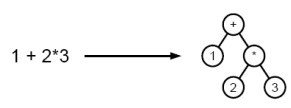
\includegraphics[,scale=1.2]{./img/1.3.jpg}
		\caption{Пример разбора выражения с преобразованием его структуры из линейной в древовидную.}  
		\label{img:1.3}
\end{figure}

В ходе синтаксического анализа исходный текст преобразуется в структуру данных, обычно — в дерево, которое отражает синтаксическую структуру входной последовательности и хорошо подходит для дальнейшей обработки. На Рисунке 1.3 представлен пример разбора выражения с преобразованием его структуры из линейной в древовидную.

\captionsetup{justification=centering,singlelinecheck=off}
\begin{figure}[h!]
	\centering
		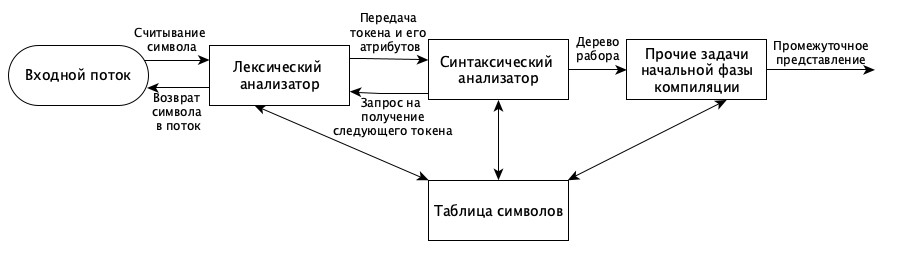
\includegraphics[,scale=0.73]{./img/1.4.jpg}
		\caption{Синтаксический анализатор.}  
		\label{img:1.4}
\end{figure}

Как правило, результатом синтаксического анализа является синтаксическое строение предложения, представленное либо в виде дерева зависимостей, либо в виде дерева разбора (см. Рисунок 1.4), либо в виде некоторого сочетания первого и второго способов представления, где каждый внутренний узел является оператором, а дочерние – его аргументами. Среди них можно выделить несколько групп связанных объектов:
\begin{itemize}[label = ---]
    \item элементы арифметических выражений: каждый узел представляет собой операцию и содержит её аргументы;
    \item элементы системы типов: базовые типы (числовые, строковые, структуры и т.п.), указатели, массивы и функции;
    \item выражения пяти типов: арифметические, блочные и управляющие выражения, условные конструкции, циклы.
\end{itemize}

Синтаксический анализатор использует следующие типы алгоритмов, выбор которого зависит от сложности и особенностей используемой грамматики:
\begin{itemize}[label = ---]
    \item Нисходящий парсер — продукции грамматики раскрываются, начиная со стартового символа, до получения требуемой последовательности токенов.
    \begin{itemize}[label = +]
        \item Метод рекурсивного спуска
        \item LL-анализатор
    \end{itemize}
    \item Восходящий парсер — продукции восстанавливаются из правых частей, начиная с токенов и заканчивая стартовым символом.
    \begin{itemize}[label = +]
        \item LR-анализатор
        \item GLR-парсер
    \end{itemize}
\end{itemize}

Перед обработчиком ошибок синтаксического анализатора стоят следующие основные задачи, сочетающие выявление ошибок и корректную обработку данных:
\begin{itemize}[label = ---]
    \item Четко и точно сообщать о наличии ошибок в анализируемой входной последовательности.
    \item Обеспечивать быстрое восстановление после обнаружения ошибки, чтобы можно было продолжить поиск других ошибок.
    \item Не замедлять существенно обработку корректной входной последовательности.
\end{itemize}


Таким образом, синтаксический анализ закладывает фундамент для всего процесса компиляции, формируя структурное представление исходной программы. Эффективная реализация синтаксического анализатора является ключевой для производительности и корректности работы компилятора в целом.

\subsection{Семантический анализатор}
Этап семантической валидации в компиляции выполняет проверку корректности смысловых связей в коде программы и собирает данные о типизации для последующего этапа компиляции — генерации исполняемого кода. Для этого используются структуры данных, сформированные на этапе синтаксического анализа, которые позволяют определить связи между операторами и операндами в выражениях и командах.

Модуль семантической валидации обычно состоит из нескольких подмодулей, каждый из которых специализируется на проверке определённого вида конструкций. Каждый подмодуль активируется синтаксическим анализатором, когда тот обнаруживает конструкцию, требующую семантической проверки.

Подмодули семантической валидации обмениваются информацией через специализированные структуры данных, такие как таблица символов, что обеспечивает их взаимодействие и координацию.


Приведем несколько общих примеров использования семантического анализатора:
\begin{itemize}[label = ---]

    \item \textbf{Проверка объявления переменных}\\
Семантический анализатор проверяет, что каждая переменная, используемая в программе, была корректно объявлена. Он отслеживает информацию о типах, областях видимости и других атрибутах переменных, хранящуюся в таблице символов.\\
Например, при обнаружении обращения к неописанной переменной, семантический анализатор сгенерирует сообщение об ошибке.
    \item \textbf{Проверка согласованности операций}\\
Семантический анализатор также проверяет, что операции, выполняемые над операндами, корректны с точки зрения их типов. \\Так, при попытке сложить число и строку, анализатор выявит несоответствие типов и сообщит об ошибке.
    \item \textbf{Проверка областей видимости}\\
Анализатор контролирует, чтобы переменные использовались только в тех областях, где они были объявлены. Он отслеживает вложенность блоков кода и правила управления областями видимости.\\
Например, при попытке обратиться к локальной переменной за пределами ее блока, анализатор сгенерирует сообщение об ошибке ”использование недоступной переменной”.
\end{itemize}

Теперь рассмотрим конкретный сложный пример с фрагментом кода, в котором используются шаблоны проектирования и обобщённое программирование (см. Листинг \ref{3}):
% \clearpage
\begin{lstlisting}[label = 3, caption =  Фрагмент кода с шаблонами проектирования и обобщенным программированием]
    #include <stdio.h>
    template<typename T>
    T max(T a, T b) {
        return a > b ? a : b;
}

int main() {
    int i = max(3, 7);
    double d = max(6.34, 3.12);
    std::string s = max(std::string("apple"), std::string("orange"));
}
\end{lstlisting}

В данном примере на этапе семантической валидации анализатор должен убедиться, что функция max может быть применена к различным типам данных. Для этого он проверяет, что оператор сравнения > поддерживается для каждого из типов T, передаваемых в функцию. Кроме того, анализатор должен проверить, что для каждого вызова функции max существуют соответствующие типы аргументов, которые могут быть сравнены, и что результат сравнения может быть возвращён из функции.

Таким образом, семантический анализатор играет ключевую роль в обеспечении смысловой корректности анализируемой программы, выявляя широкий спектр логических ошибок на ранних этапах трансляции.

\subsection{Генерация кода}
Последний этап – генерация кода. Начинается тогда, когда во все системные таблицы занесена необходимая информация. В этом случае, компилятор переходит к построению соответствующей программы в машинном коде. Код генерируется при обходе дерева разбора, построенного на предыдущих этапах.

Для получения машинного кода требуется два отдельных прохода:
\begin{itemize}[label = ---]
    \item генерация промежуточного кода;
    \item генерация собственно машинного кода.
\end{itemize}

Для каждого узла дерева генерируется соответствующий операции узла код на целевой платформы. В процессе анализа кода программы данные связываются с именами переменных. При выполнении генерации кода предполагается, что вход генератора не содержит ошибок. Результат – код, пригодный для исполнения на целевой платформе.

В качестве примера рассмотрим трансляцию следующего выражения \\$a = b * -c + b * -c$ в промежуточный и машинный код. Предположим, что переменные a, b, и c уже определены и расположены в памяти.

\begin{lstlisting}[label = 4, caption =  Шаг 1. Генерация промежуточного кода. Выражение преобразуется
в последовательность трехадресных инструкций]
t1 = -c
t2 = b * t1
t3 = -c
t4 = b * t3
a = t2 + t4
\end{lstlisting}
\clearpage
\begin{lstlisting}[label = 5, caption = Шаг 2. Оптимизация промежуточного кода. Устраняем повторяющиеся вычисления]
t1 = -c
t2 = b * t1
a = t2 + t2
\end{lstlisting}

\begin{lstlisting}[label = 6, caption = Шаг 3. Генерация машинного кода. Промежуточный код транслируется в инструкции для конкретной целевой машины]
LOAD R1, c
NEG R1
MUL R2, b, R1
ADD R3, R2, R2
STORE a, R3
\end{lstlisting}

Этот пример иллюстрирует ключевые этапы трансляции: от промежуточного представления выражений до их физического выполнения на аппаратном уровне.

\section{Методы реализации лексического и синтаксического анализаторов}
В современной разработке компиляторов применяются разнообразные методы для создания лексических и синтаксических анализаторов. Эти методы можно классифицировать как:

\begin{itemize}[label = ---]
    \item Традиционные алгоритмы, основанные на проверенных временем техниках;
    \item Современные инструменты, автоматизирующие процесс генерации.
\end{itemize}

\subsection{Генераторы лексического анализатора}
На рынке представлено множество инструментов для генерации лексических анализаторов, среди которых выделяются Lex, Flex, ANTLR4 и другие. \cite{2}

\textbf{Lex}: Этот инструмент является классическим решением в среде Unix и часто используется в паре с Yacc для создания синтаксических анализаторов. Lex обрабатывает входные данные и генерирует исходный код на C, структурированный в три секции: определения, правила и код на C.

\textbf{Flex}: Как усовершенствованная версия Lex, Flex используется в GNUсистемах и предлагает схожую функциональность.

\textbf{ANTLR4}: Этот инструмент поддерживает широкий спектр языков программирования и обеспечивает генерацию классов для рекурсивного нисходящего синтаксического анализа. ANTLR4 позволяет создавать анализаторы, основанные на РБНФ грамматике, и предоставляет возможности для построения и обхода деревьев анализа.

Сравнение инструментов для лексического анализа выделяет ANTLR4 как наиболее предпочтительный инструмент по следующим причинам:
\begin{itemize}[label = ---]
    \item Универсальность: ANTLR4 поддерживает широкий спектр целевых языков программирования, что делает его идеальным выбором для проектов, требующих кросс-платформенной совместимости. \cite{4}
    \item Продвинутые возможности: В отличие от Lex и Flex, ANTLR4 предлагает более продвинутые возможности для работы с грамматикой, включая поддержку РБНФ, что позволяет создавать более сложные и мощные анализаторы.
    \item Простота использования: ANTLR4 упрощает процесс разработки анализаторов благодаря интуитивно понятным абстракциям и шаблонам, что сокращает время разработки и упрощает поддержку кода.
    \item Эффективность: Генерируемые ANTLR4 анализаторы характеризуются высокой производительностью и оптимизацией, что критически важно для компиляторов и других инструментов анализа кода.
\end{itemize}
    
В то время как Lex и Flex остаются надежными инструментами, особенно в Unix-подобных системах, их функциональность ограничена по сравнению с ANTLR4. ANTLR4 предоставляет более широкие возможности и гибкость, что делает его предпочтительным выбором для современных проектов по созданию лексических и синтаксических анализаторов.

\subsection{Генераторы синтаксического анализатора}
В сфере разработки парсеров ключевым аспектом является выбор инструментария, который определяет эффективность и гибкость создаваемого решения. В этом контексте выделяются следующие инструменты:

\textbf{Yacc/Bison}: Эти генераторы парсеров трансформируют грамматические определения в исполняемый код на C, обеспечивая интеграцию с системами Unix (Yacc) и GNU (Bison). \cite{5}

\textbf{Coco/R}: Платформа для генерации парсеров, поддерживающая множество языков программирования, включая C++ и Java, использует концепции конечных автоматов для лексического анализа и рекурсивного спуска для синтаксического.

Применение конечных автоматов позволяет лексическим анализаторам эффективно распознавать лексемы, в то время как рекурсивный спуск обеспечивает точность синтаксического анализа, необходимую для обработки вложенных структур и сложных грамматик. ANTLR, интегрируя эти методы, предоставляет разработчикам мощный инструментарий для создания высокопроизводительных парсеров, способных работать с разнообразными грамматическими конструкциями.

\section{LLVM}
LLVM (Low Level Virtual Machine) – проект программной инфраструктуры для создания компиляторов и сопутствующих им утилит. В его основе лежит платформонезависимая система кодирования машинных инструкций – байткод LLVM IR (Intermediate Representation). LLVM может создавать байткод для множества платформ, включая ARM, x86, x86-64, GPU от AMD и Nvidia и другие. В проекте есть генераторы кода для множества языков, а для компиляции LLVM IR в код платформы используется clang. В состав LLVM входит также интерпретатор LLVM IR, способный исполнять код без компиляции в код платформы. \cite{6}
 
Некоторые проекты имеют собственные LLVM-компиляторы, например, LLVM-версия GCC.

LLVM поддерживает целые числа произвольной разрядности, числа с плавающей точкой, массивы, структуры и функции. Большинство инструкций в LLVM принимает два аргумента (операнда) и возвращает одно значение (трёхадресный код).

Значения в LLVM определяются текстовым идентификатором. Локальные значения обозначаются префиксом \%, а глобальные – @. Тип операндов всегда указывается явно и однозначно определяет тип результата. Операнды арифметических инструкций должны иметь одинаковый тип, но сами инструкции «перегружены» для любых числовых типов и векторов.

LLVM поддерживает полный набор арифметических операций, побитовых логических операций и операций сдвига. LLVM IR строго типизирован, 18поэтому существуют операции приведения типов, которые явно кодируются специальными инструкциями. Кроме того, существуют инструкции преобразования между целыми числами и указателями, а также универсальная инструкция для приведения типов bitcast.

Помимо значений регистров в LLVM есть работа с памятью. Значения в памяти адресуются типизированными указателями. Обратиться к ней можно с помощью двух инструкций: load и store. Инструкция alloca выделяет память на стеке. Она автоматически освобождается при выходе из функции при помощи
инструкций ret или unwind.

Для вычисления адресов элементов массивов и структур с правильной типизацией используется инструкция getelementptr. Она только вычисляет адрес без обращения к памяти, принимает произвольное количество индексов и может разыменовывать структуры любой вложенности.

\section*{Выводы}
В данном разделе приведён обзор основных фаз компиляции, описана каждая из них. Также был выбран генератор лексического и синтаксического анализаторов – ANTLR и LLVM в качестве генератора машинного кода.